\chapter{Deep Equilibrium Methods}\label{ch:deq}

Most modern feedforward deep networks and unrolled architectures are built upon the core concept of explicitly stacked layers \cite{bai2019deep}. In the forward pass, these networks consist of a sequence of $L$ transformations, where $L$ defines the depth of the network or the number of unrolled algorithmic iterations. To optimise these networks, the backward pass relies on backpropagating errors through the exact same $L$ layers via the chain rule \cite{rumelhart1986learning}. Consequently, this necessitates storing the intermediate activation values of every single layer, creating an $\mathcal{O}(L)$ memory bottleneck that strictly limits the capacity, resolution, and depth of the models that can be trained on modern hardware \cite{bai2019deep, kolter2020deepimplicit}. Furthermore, utilising a fixed, pre-determined number of layers $L$ restricts flexibility. If an unrolled model requires more iterations to converge at inference time than it was trained for, it often suffers from severe truncation errors and mathematical instability. This is precisely the trade-off that began to emerge in Chapter \ref{ch:unrolling}. Finite unrolling gives interpretable, trainable architectures, but ties accuracy, memory, and depth directly to the chosen iteration budget.

To overcome these limitations, recent research has shifted toward continuous dynamics and implicit models. While Deep Equilibrium (DEQ) models have recently demonstrated highly competitive performance relative to state-of-the-art explicit models across various domains, the foundational idea is not entirely new \cite{bai2019deep}. The concept of specifying a layer that finds the fixed point of an iterative procedure traces its roots back to the late 1980s with the introduction of recurrent backpropagation \cite{almeida1987learning, pineda1987generalization}. These early works recognised that network states could be driven to an equilibrium, though they were typically restricted to small-scale, fixed-input settings and lacked the architectural complexity of modern deep learning. Conceptually, this also aligns with Chapter \ref{ch:pnp}. Once we move to operator-based viewpoints, fixed points and equilibrium conditions become central objects rather than side effects of finite algorithms.

The modern DEQ framework represents a significant evolution of these classical concepts \cite{bai2019deep, kolter2020deepimplicit}. Instead of passing data through a finite sequence of explicitly defined algebraic transformations, DEQs attempt to express the entire deep architecture as a single, infinitely deep, weight-tied equilibrium computation. More crucially, rather than relying solely on naive, slow fixed-point iteration to reach this state, DEQs utilise highly efficient black-box root-finding algorithms, such as Broyden's method \cite{broyden1965class} or Anderson acceleration \cite{walker2011anderson}, to solve for the fixed point directly \cite{kolter2020deepimplicit}. By framing the forward pass as a root-finding problem, the model output becomes agnostic to the specific solver trajectory. This removes the need to store intermediate states and decouples representational depth from memory footprint. In that sense, DEQs complement Chapter \ref{ch:continuous_dynamics}. Where continuous-depth models reinterpret layers through ODE flows and optimal control, DEQs reinterpret depth through equilibrium states and implicit differentiation.

Figure \ref{fig:deq_memory_footprint} provides a visual comparison of this memory argument. Explicit architectures incur memory growth with depth, whereas DEQs retain a constant memory footprint by solving directly for the equilibrium state.

\begin{figure}[htpb]
    \centering
    \begin{minipage}{0.35\textwidth}
        \centering
        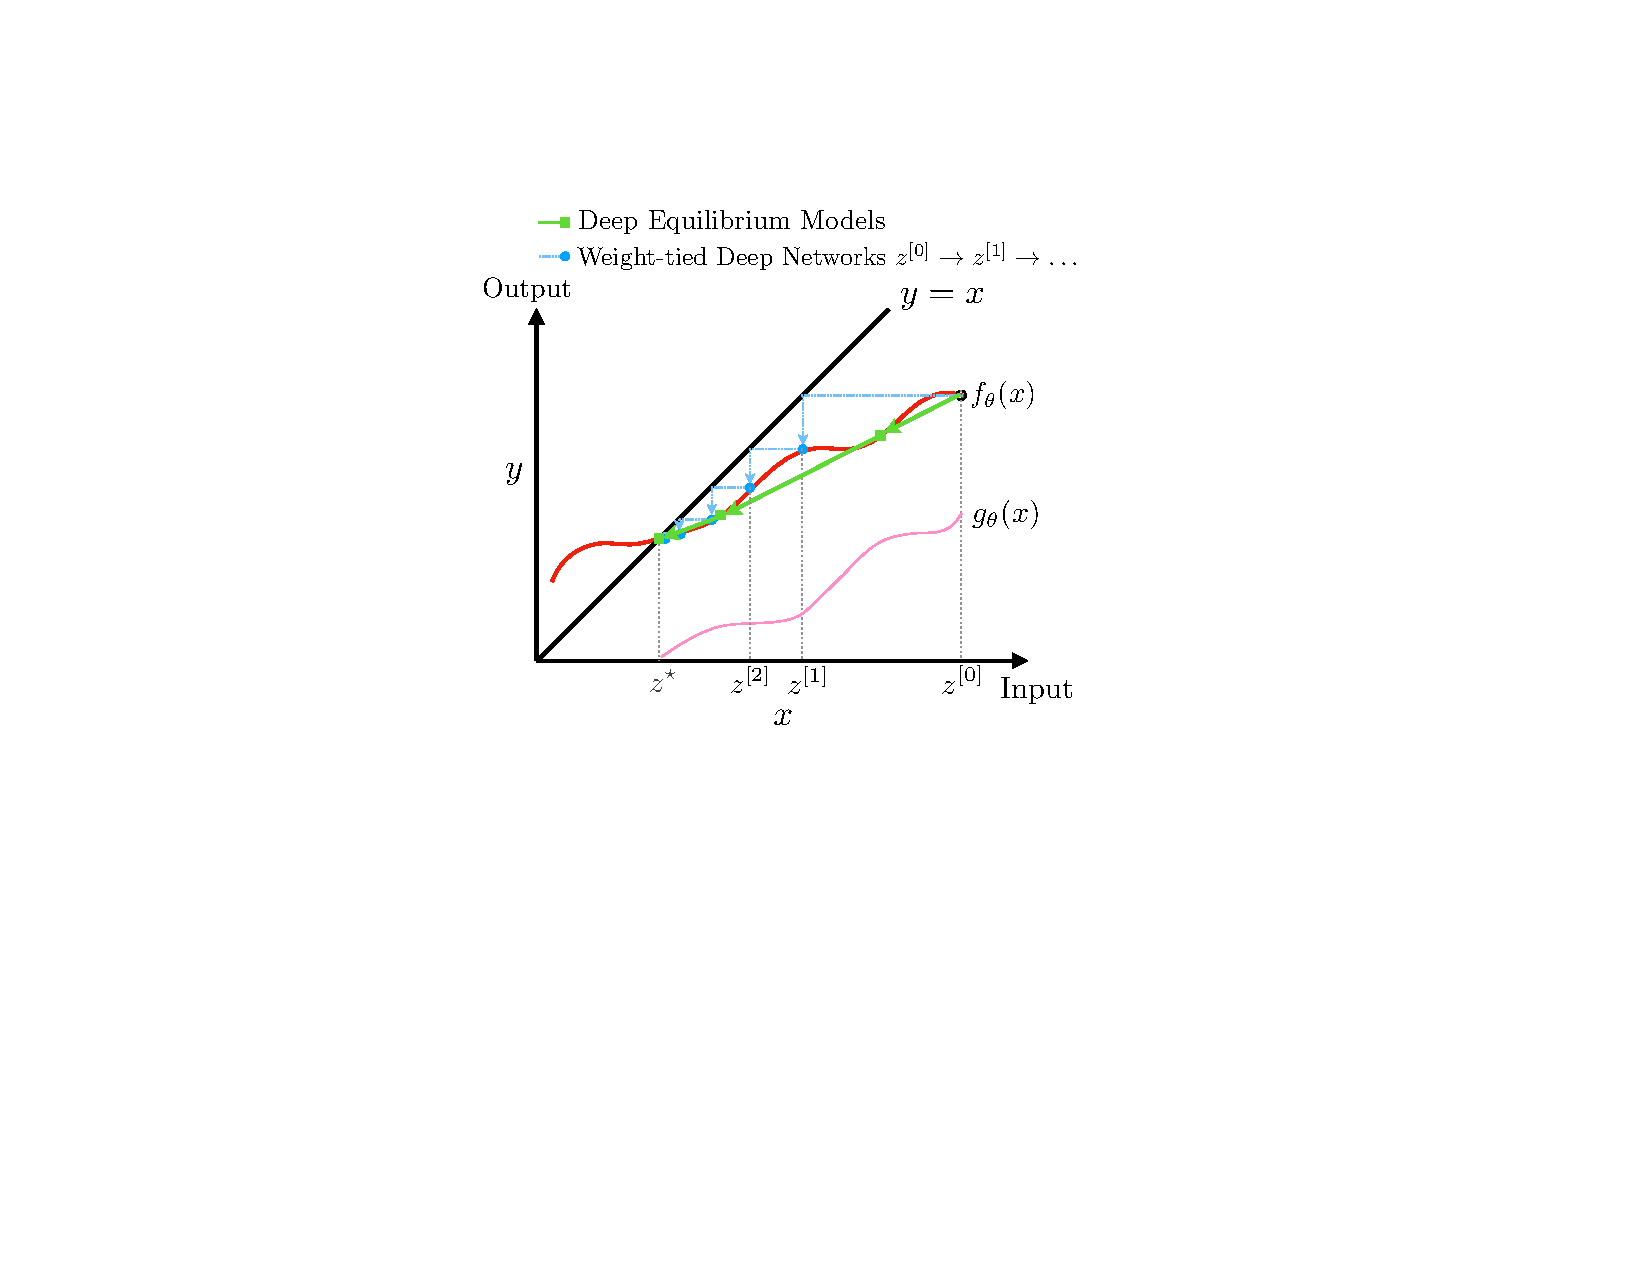
\includegraphics[width=\textwidth]{../Common_Images/deq/fp_onefig.pdf}
        \caption*{Solving for an equilibrium point in 2D.}
    \end{minipage}
    \hfill
    \begin{minipage}{0.62\textwidth}
        \centering
        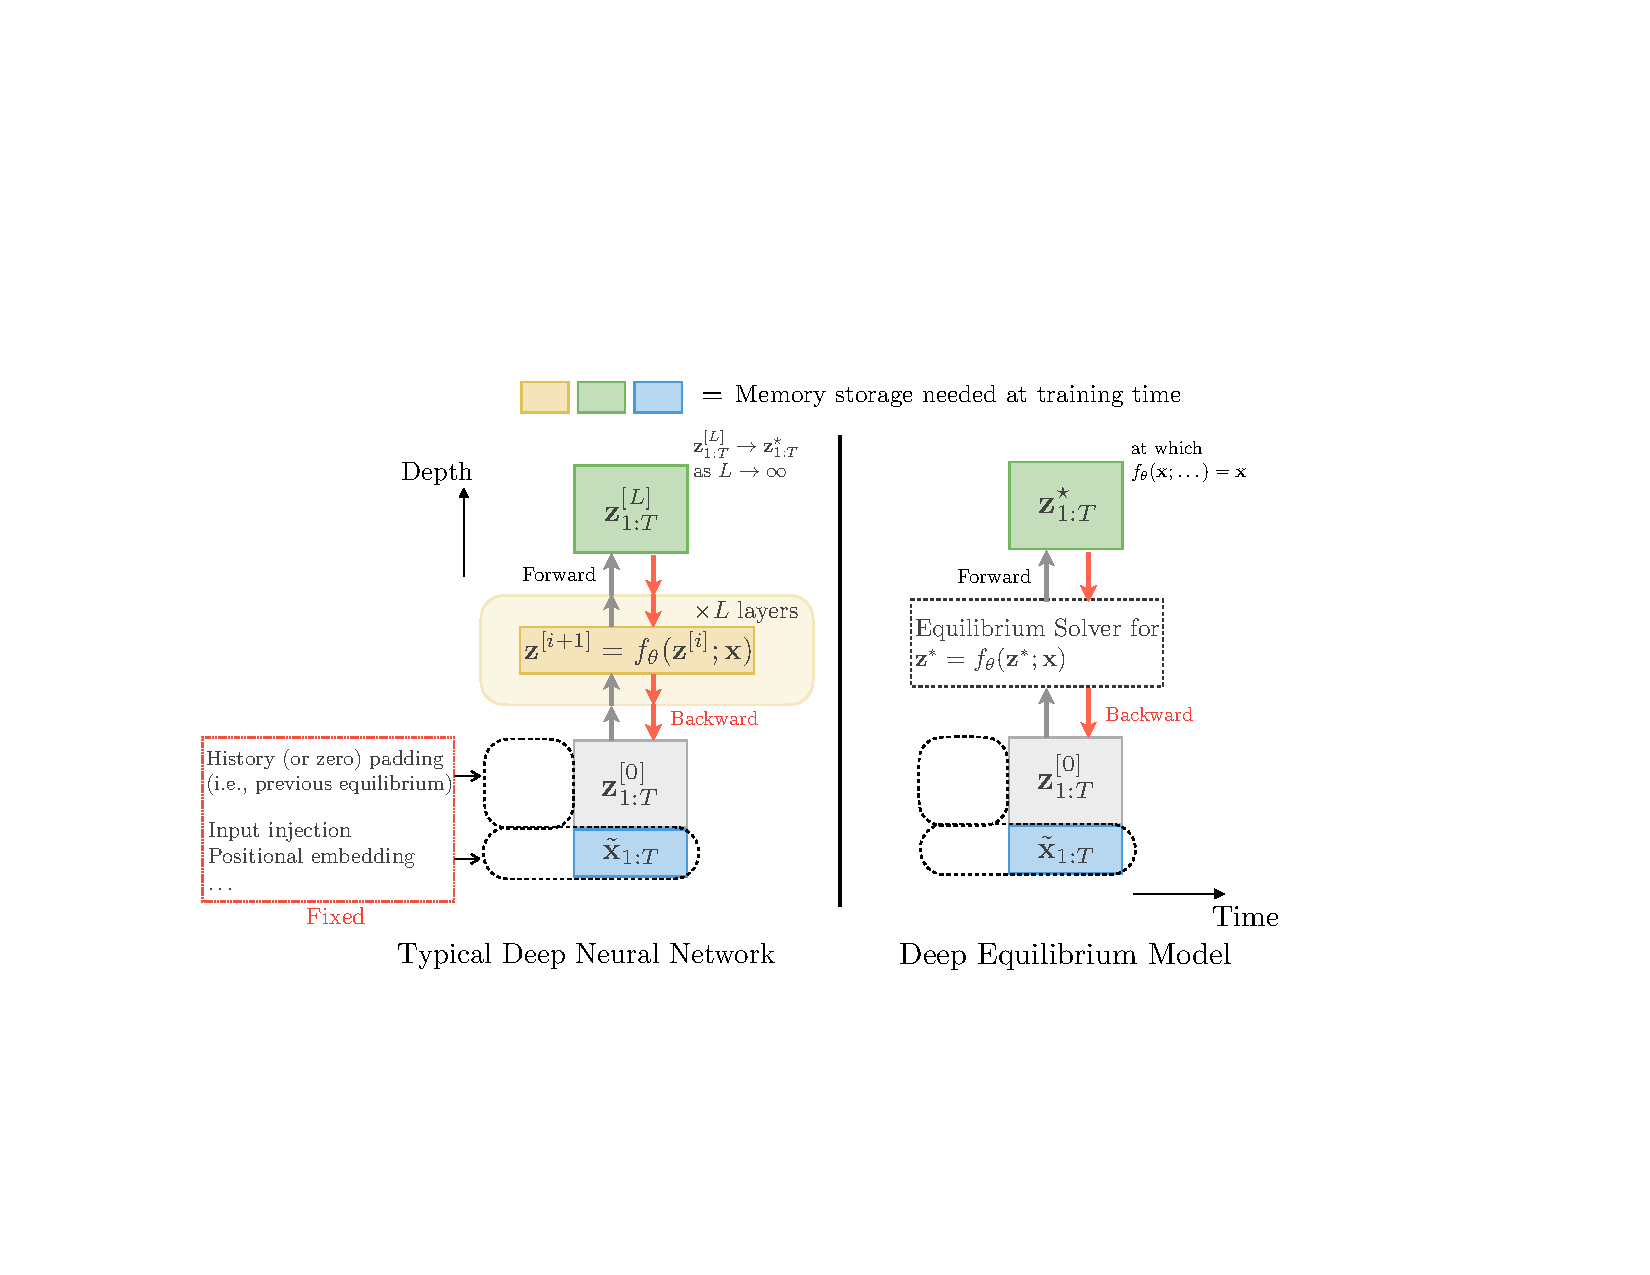
\includegraphics[width=\textwidth]{../Common_Images/deq/equm_vs_dnn.pdf}
        \caption*{DEQ vs conventional deep network memory.}
    \end{minipage}
    \caption{Comparison of memory consumption and dynamics in explicit deep networks and Deep Equilibrium models. Explicit layer stacking requires storing intermediate activations, yielding memory growth with depth, while DEQs compute an equilibrium state with constant memory usage. From \cite{bai2019deep}.}
    \label{fig:deq_memory_footprint}
\end{figure}

\section{The Equilibrium Equation}
To understand implicit models, we shift our perspective from sequential layer composition to steady states of an operator. In an explicit network as introduced in Section \ref{sec:deep-learning}, one may write layer transitions as
\begin{equation}
    z_{i+1} = f_{\theta_i}(z_i, x).
    \label{eq:deq-fp-v1}
\end{equation}
Here, $x$ denotes the network input, $z_i$ the hidden state at layer (or iteration) $i$, $\theta_i$ the parameters of the $i$th transformation, and $f_{\theta_i}$ the corresponding update map. If weights are tied across depth, this becomes repeated application of the same map $f_\theta$. An equilibrium state $z^\star$ then satisfies the fixed-point condition
\begin{equation}
    z^\star = f_\theta(z^\star, x).
    \label{eq:deq_fixed_point_v1}
\end{equation}

This mirrors the fixed-point structure already encountered in Chapter \ref{ch:pnp}, where PnP-HQS is written as an operator iteration in Equation \eqref{eq:pnp_hqs_operator}. The direct approach to this is fixed-point iteration but this time with fixed parameters, i.e.
\begin{equation*}
    z_{i+1} = f_\theta(z_i, x),
\end{equation*}
which converges under suitable assumptions. As discussed in Section \ref{sec:pnp_convergence}, convergence follows from Banach's fixed-point theorem for strict contractions, and can still be established for relaxed iterations of non-expansive maps via Krasnosel'skii-Mann theory. Note that DEQs typically recast Equation \eqref{eq:deq_fixed_point_v1} as a root-finding problem,
\begin{equation}
    g_\theta(z^\star, x) := f_\theta(z^\star, x) - z^\star = 0,
    \label{eq:deq_root_v1}
\end{equation}
which is then solved with accelerated black-box methods.

\subsection{Representational Power (Universality)}
A natural concern is that replacing explicit depth by one implicit equilibrium condition might reduce expressivity. However, the opposite is true. The DEQ perspective separates \emph{how} a representation is computed from \emph{what} representation is admissible at equilibrium. This separation allows a single implicit layer to encode transformations that would otherwise be written as many explicit layers.

The first universality statement is that explicit depth can be absorbed into state dimension without exponential parameter growth. Intuitively, one embeds a finite-depth computation into a larger state, routes information between state blocks by a shared map, and recovers the explicit network output from one component of the equilibrium state.

\begin{cor}[Representational Corollary for a Single DEQ Layer \cite{bai2019deep}]
\label{cor:deq_universality_v1}
Consider a finite feedforward network of arbitrary depth and connectivity acting on input $x$. There exists a DEQ map $f_\theta(\cdot; x)$ on an augmented hidden state such that the corresponding equilibrium state $z^\star$ encodes the same input-output mapping, while the parameter count increases at most polynomially (in common constructions, linearly in the required state augmentation), and in particular does not incur exponential blowup.
\end{cor}

The second statement concerns stacking DEQ blocks. Suppose one defines two implicit layers in sequence, such that
\begin{equation*}
    z^\star = f_{\theta_1}(z^\star; x),
    \qquad
    y^\star = h_{\theta_2}(y^\star; z^\star).
\end{equation*}
If we define a joint state $s = (z,y)$ and a joint map via
\begin{equation*}
    \Gamma_\Theta(s; x)
    := \big(f_{\theta_1}(z; x),\, h_{\theta_2}(y; z)\big),
    \qquad \Theta := (\theta_1,\theta_2),
\end{equation*}
one sees that the stacked system is equivalent to a single equilibrium condition
\begin{equation*}
    s^\star = \Gamma_\Theta(s^\star; x).
\end{equation*}
Hence stacking DEQs does not enlarge the function class beyond that of a sufficiently expressive single DEQ on a larger state space.

\begin{cor}[No Additional Expressive Power from Stacking DEQs \cite{bai2019deep}]
\label{thm:deq_no_stack_gain_v1}
For DEQ layers with compatible state spaces and well-defined equilibria, any finite stack of DEQ blocks can be rewritten as one DEQ block on a concatenated hidden state. Therefore, stacked DEQs provide no additional representational power over a single DEQ layer of adequate width.
\end{cor}

In practice, this result shifts architectural emphasis away from macroscopic stacking and towards the design of a strong transformation cell $f_\theta$, including stabilisation, input injection, and inductive-bias choices appropriate for the task domain.

\section{Forward and Backward Passes in DEQs}

Having established the representational capacity of Deep Equilibrium Models to encapsulate arbitrary depth in a single fixed-point condition, we now turn to the practical mechanics of evaluating and training these models. Effectively solving the equilibrium equation requires two distinct phases: finding the fixed point during the forward pass, and computing the gradients via the adjoint method during the backward pass.

\subsection{Forward Pass (Root-Finding)}
Because the output of a DEQ is simply the equilibrium point, the forward pass can utilise any black-box root-finding algorithm to solve
\begin{equation*}
    g_\theta(z^\star; x) = f_\theta(z^\star; x) - z^\star = 0.
\end{equation*}
Naive forward iteration can work, but quasi-Newton methods such as Broyden's method and acceleration schemes such as Anderson acceleration typically converge much faster in practice.

For this to be well posed, one needs existence of an equilibrium, and for robust computation typically uniqueness and local stability of the iteration map. In inverse-problem DEM constructions (for example DE-GRAD, DE-PROX, DE-ADMM that we will introduce in Section \ref{sec:dem}), these properties are enforced by Lipschitz and step-size conditions that make the map contractive. Under standard fixed-point iteration (also known as Picard iteration), defined as $z_{k+1} = f_\theta(z_k; x)$, local convergence is guaranteed if the spectral radius of the Jacobian $\rho(J_{f_\theta}) < 1$, yielding convergence by Banach's fixed-point theorem \cite{gilton2021deep, riccio2022regularization}.

\subsubsection*{Broyden and Limited-Memory Broyden}

While Picard iteration provides theoretical guarantees for strictly contractive mappings, its linear convergence rate is often too slow for practical deep learning applications. A more efficient strategy shifts from fixed-point iteration to root-finding by seeking the root of the residual function $g_\theta(z; x) = z - f_\theta(z; x) = 0$. The natural tool for this is Newton's method, which leverages first-order derivative information via the Jacobian matrix $J_{g_\theta} = \partial_z g_\theta$, containing all first-order partial derivatives of the vector-valued function $g_\theta$. Newton's method would update via
\begin{equation*}
    z_{k+1} = z_k - J_{g_\theta}(z_k;x)^{-1} g_\theta(z_k;x),
\end{equation*}
but explicitly forming and inverting the $d \times d$ Jacobian matrix $J_{g_\theta}$ is computationally infeasible at the scale of modern deep neural networks. Broyden's method circumvents this by acting as a \emph{quasi-Newton} method, replacing the exact inverse Jacobian with an iterative approximation $H_k \approx J_{g_\theta}(z_k;x)^{-1}$.

To understand where this approximation originates, we can look at the generalisation of the 1D secant method. In one dimension, the derivative is approximated via finite differences: $f'(x_k) \approx \frac{f(x_k) - f(x_{k-1})}{x_k - x_{k-1}}$. In multiple dimensions, defining $\Delta z_k := z_k-z_{k-1}$ and $\Delta g_k := g_k-g_{k-1}$ where $g_k := g_\theta(z_k;x)$, the equivalent condition on the approximated Jacobian $B_k \approx J_{g_\theta}$ is the secant equation $B_k \Delta z_k = \Delta g_k$. Multiplying both sides by the inverse approximation $H_k = B_k^{-1}$ yields the inverse secant condition
\begin{equation*}
    H_k \Delta g_k = \Delta z_k.
\end{equation*}
However, because this imposes only $d$ equations on a $d \times d$ matrix, the system is dramatically underdetermined. Broyden resolved this by proposing that the updated matrix $H_k$ should satisfy the secant equation while deviating as little as possible from the previous estimate $H_{k-1}$. Mathematically, this is framed as a constrained optimisation problem minimising the Frobenius norm (often squared for mathematical convenience), i.e.,
\begin{equation*}
    \min_{H_k} \frac{1}{2}\|H_k - H_{k-1}\|_F^2 \quad \text{subject to} \quad H_k \Delta g_k = \Delta z_k.
\end{equation*}
To solve this constrained minimisation problem, we introduce a Lagrange multiplier vector $\lambda \in \mathbb{R}^d$ and define the Lagrangian
\begin{equation*}
    \mathcal{L}(H_k, \lambda) = \frac{1}{2}\|H_k - H_{k-1}\|_F^2 + \langle \lambda, \Delta z_k - H_k \Delta g_k \rangle.
\end{equation*}
Setting the gradient with respect to the matrix $H_k$ to zero gives the optimality condition
\begin{equation*}
    \nabla_{H_k} \mathcal{L} = H_k - H_{k-1} - \lambda \Delta g_k^{\top} = 0 
    \quad \implies \quad 
    H_k = H_{k-1} + \lambda \Delta g_k^{\top}.
\end{equation*}
This explicitly reveals that the minimal-distance update is inherently a rank-one matrix. By substituting this deduced form back into the secant constraint $H_k \Delta g_k = \Delta z_k$, we can explicitly solve for the multiplier $\lambda$ to obtain
\begin{equation*}
    (H_{k-1} + \lambda \Delta g_k^{\top})\Delta g_k = \Delta z_k 
    \quad \implies \quad 
    \lambda \|\Delta g_k\|_2^2 = \Delta z_k - H_{k-1}\Delta g_k.
\end{equation*}
Isolating $\lambda$ and substituting it back into the update equation for $H_k$ directly yields the recursive rank-one update
\begin{equation*}
    H_k
    = H_{k-1}
    + \frac{(\Delta z_k-H_{k-1}\Delta g_k)\,\Delta g_k^{\top}}{\|\Delta g_k\|_2^2}
    = H_{k-1} + (\Delta z_k-H_{k-1}\Delta g_k)\,(\Delta g_k)^\dagger,
\end{equation*}
where $(\Delta g_k)^\dagger = \Delta g_k^{\top}/\|\Delta g_k\|_2^2$ is the Moore-Penrose pseudoinverse of the nonzero vector $\Delta g_k$. Notice that the term $(\Delta z_k-H_{k-1}\Delta g_k)\,(\Delta g_k)^\dagger$ forms an outer product of two vectors, defining a rank-one matrix. This rank-one update modifies the inverse Jacobian approximation $H_{k-1}$ just enough to satisfy the secant equation in the direction of the recent step, while leaving its behaviour in orthogonal directions entirely unchanged.

A crucial computational detail often missed is how this is applied in practice. Computing the update step $z_{k+1} = z_k - H_k g_k$ does not actually require instantiating the dense $d \times d$ matrix $H_k$ in memory. Because $H_k$ is constructed entirely from successive rank-one updates starting from an initial guess (such as $H_0 = -I$), the matrix-vector product $H_k g_k$ can be evaluated efficiently using only vector inner products. 

In DEQ implementations, this is pushed further by using Limited-memory Broyden (L-Broyden) variants. Instead of implicitly rolling up all $k$ historical updates, the algorithm stores only the most recent $m$ secant pairs $\{(\Delta z_i, \Delta g_i)\}_{i=k-m+1}^k$. Older secant pairs are seamlessly discarded, bringing the memory footprint from $\mathcal{O}(d^2)$ purely down to $\mathcal{O}(md)$, all while retaining critical quasi-Newton curvature information \cite{broyden1965class, bai2019deep}. Unlike Picard or Banach iterations which strictly require $\rho(J_{f_\theta}) < 1$, Broyden's method only requires that the residual's Jacobian is non-singular (i.e., $1$ is not an eigenvalue of $J_{f_\theta}$) and that the initial guess is sufficiently close to the true fixed point. This flexibility allows it to converge efficiently even for mappings where simple fixed-point iterations would diverge.

\subsubsection*{Anderson Acceleration and Its Link to Broyden}
Anderson acceleration (AA) starts from the fixed-point iteration rather than a Newton update: one forms an affine combination of recent iterates that minimises the current residual in a small least-squares problem \cite{walker2011anderson}. Storing residuals $g_i=g_\theta(z_i;x)$ and collecting recent differences in
\begin{equation*}
    S_k := [\Delta z_{k-m+1},\ldots,\Delta z_k],
    \qquad
    Y_k := [\Delta g_{k-m+1},\ldots,\Delta g_k],
\end{equation*}
the most common AA form used for DEQ fixed-point iterations is
\begin{equation*}
    z_{k+1}^{\mathrm{AA}}
    = z_k + g_k - (S_k+Y_k)\gamma_k,
    \qquad
    \gamma_k \in \arg\min_{\gamma}\|g_k-Y_k\gamma\|_2^2,
\end{equation*}
hence (for full-column-rank or pseudoinverse solution) we have $\gamma_k = Y_k^\dagger g_k$.

This exposes the algebraic link to multisecant quasi-Newton updates: AA can be interpreted as a multisecant Broyden-type step, and in the full-memory, untruncated setting with initial inverse guess $H_0=-I$, the resulting update has the same form as the corresponding multisecant inverse-Broyden step. Conceptually, Broyden and AA differ in derivation, but both exploit low-dimensional secant subspaces and small least-squares/pseudoinverse solves to accelerate equilibrium computation. Furthermore, when Anderson Acceleration is applied to a strictly linear system, it becomes mathematically equivalent to the Generalised Minimal Residual method (GMRES), a highly robust Krylov subspace iterative solver. This connection becomes particularly important for the adjoint computations during the backward pass.

\subsection{Backward Pass (Implicit Differentiation)}

Rather than backpropagating through the sequence of forward root-finder iterations, DEQs obtain gradients analytically by taking the transpose of implicit differentiation. An elegant way to derive this is by formulating the backward pass as a constrained optimisation problem. Suppose we want to minimise an empirical risk loss objective $\mathcal{L}_{\text{task}}(z, \theta)$ with the DEQ equilibrium condition serving as the equality constraint. The Lagrangian formulation reads
\begin{equation*}
    \mathcal{L}(z, \theta; v) = \mathcal{L}_{\text{task}}(z, \theta) - \langle v, z - f_\theta(z; x) \rangle,
\end{equation*}
where $v$ serves as the dual variable or adjoint state (the negative sign on the inner product serves to match the typical sign combinations in DEQ literature). To find the adjoint equation, we evaluate the stationary point of the Lagrangian with respect to the hidden state $z$. According to the Karush-Kuhn-Tucker (KKT) conditions, at the optimal state (the fixed point $z^\star$), the gradient with respect to $z$ must vanish, i.e.,
\begin{equation*}
    \nabla_z \mathcal{L}(z^\star, \theta; v) = \nabla_z \mathcal{L}_{\text{task}}(z^\star, \theta) - v + (\partial_z f_\theta(z^\star; x))^{\top} v = 0.
\end{equation*}
Rearranging this gives a direct fixed-point condition for the adjoint variable $v$. Denoting the forward Jacobian transpose evaluated at the equilibrium point as $J_{f_\theta}^{\top} = (\partial_z f_\theta(z^\star; x))^{\top}$, we obtain
\begin{equation*}
    (I - J_{f_\theta}^{\top}) v = \nabla_z \mathcal{L}_{\text{task}}(z^\star, \theta) 
    \quad \Longleftrightarrow \quad
    v = J_{f_\theta}^{\top} v + \nabla_z \mathcal{L}_{\text{task}}(z^\star, \theta).
\end{equation*}
This explicitly derives the IFT logic used in Section \ref{sec:bilevel}, matching Equation \eqref{eq:bilevel_sensitivity}. Once the adjoint state $v$ converges, we can calculate the total derivative of the loss with respect to the continuous parameters $\theta$ by differentiating the Lagrangian directly to obtain
\begin{equation*}
    \frac{\partial \mathcal{L}_{\text{task}}}{\partial \theta} = \nabla_\theta \mathcal{L}(z^\star, \theta; v) = \nabla_\theta \mathcal{L}_{\text{task}}(z^\star, \theta) + \left\langle v, \partial_\theta f_\theta(z^\star; x) \right\rangle.
\end{equation*}
Typically, $\mathcal{L}_{\text{task}}$ evaluates on the final state and has no explicitly separate parameterisation in $\theta$, meaning $\nabla_\theta \mathcal{L}_{\text{task}}(z^\star, \theta) = 0$. In this case, the gradient simplifies strictly to $\langle v, \partial_\theta f_\theta(z^\star; x) \rangle$, aligning with standard formulations \cite{bai2019deep, riccio2022regularization}.

\subsection{Constant Memory Footprint and Convergence Guarantees}
The central computational step in the backward pass is a vector-Jacobian product inside the linear solve for $v$, completely avoiding the need to retain intermediate forward trajectory states $z_k$. The adjoint $v$ is evaluated iteratively by accelerated solvers such as Broyden's method, Anderson Acceleration or a Neumann series, mimicking the forward equilibrium calculation \cite{bai2019deep, gilton2021deep}. As a result, the training memory maintains an $\mathcal{O}(1)$ footprint regardless of effective algorithm depth, drastically reducing demands compared to $\mathcal{O}(L)$ memory in depth-$L$ explicit models.

A remarkable mathematical synergy arises when guaranteeing convergence for both the forward and backward passes. Because the linear operator driving the adjoint iteration is explicitly $J_{f_\theta}^{\top}$, it shares exactly the same eigenvalues as the forward Jacobian $J_{f_\theta}$. Thus, their spectral radii remain identical, $\rho(J_{f_\theta}^{\top}) = \rho(J_{f_\theta})$. Therefore, if the forward pass converges as a strict contraction mapping (guaranteeing $\rho < 1$ for Picard iteration), the adjoint pass is automatically guaranteed to be a contraction with the exact same theoretical convergence rate.

When employing robust quasi-Newton solvers such as Broyden's method or Anderson Acceleration, the strict contraction requirement drops. For these methods to successfully find a root, the true Jacobian of the residual $I - J_{f_\theta}$ merely needs to be non-singular—indicating that $1$ is an excluded eigenvalue of $J_{f_\theta}$. By the same transpose property, $I - J_{f_\theta}^{\top}$ inherently also avoids singularity, guaranteeing a unique solution for the adjoint state. Because the adjoint equation is strictly linear with respect to $v$, iterative solvers are unburdened with local proximity restrictions. Applying Anderson Acceleration effectively executes GMRES algorithms on a linear system, guaranteeing the system approaches the exact adjoint variable $v$ from the initial guess (typically initialised to zero).

\section{Application 1: Deep Sequence Modelling}
Deep Equilibrium models are particularly natural for sequence learning, where explicit depth is often used as a proxy for iterative refinement of temporal representations. In the DEQ view, this refinement is sent to its limit and represented directly by the equilibrium condition $z^\star = f_\theta(z^\star, x)$,
so the model output is defined by a fixed point rather than by a finite stack of layers. As discussed in the original DEQ work and in this \href{https://implicit-layers-tutorial.org/deep_equilibrium_models/}{implicit-layers tutorial}, this interpretation is not tied to a specific cell design: one may choose any stable sequence cell $f_\theta$, and use root-finding to obtain the same equilibrium state that an infinitely deep weight-tied architecture would approach \cite{bai2019deep, kolter2020deepimplicit}.

Two concrete instantiations are especially important. First, DEQ-TrellisNet uses weight-tied temporal convolutions with input injection, preserving causal sequence processing while replacing explicit unrolling by equilibrium computation. Second, DEQ-Transformer uses weight-tied multi-head self-attention (with normalisation and positional information) inside the same equilibrium framework. In both cases, input injection is essential; because the equilibrium is independent of any particular initial iterate, the map must include the input at each update so that $z^\star$ remains a function of $x$ rather than collapsing to an input-agnostic fixed point \cite{bai2019deep, kolter2020deepimplicit}.

Empirically, these models are competitive with, and in several settings slightly better than, strong explicit-depth baselines of similar parameter count. On the long-range copy-memory task (delay $T=400$), DEQ-Transformer achieves substantially lower loss than recurrent baselines, confirming strong long-term retention. On the word-level Penn Treebank benchmark, DEQ-TrellisNet achieves test perplexity comparable to deep TrellisNet while avoiding layerwise storage overhead. On the larger WikiText-103 benchmark, DEQ-TrellisNet and DEQ-Transformer variants match or improve corresponding TrellisNet/Transformer-XL configurations at similar non-embedding model sizes \cite{bai2019deep}.

The key practical gain is memory efficiency. Since gradients are computed by implicit differentiation and linear fixed-point solves, training memory is approximately constant with respect to effective depth. In the original sequence experiments, this translated into over 80\% memory savings, with reductions up to 88\% relative to deep stacked baselines, and still substantial savings even against gradient-checkpointed models \cite{bai2019deep}. This changes the deployment regime for sequence models: capacities that previously required aggressive memory engineering or multi-device training can often be handled on a single accelerator. The main trade-off is runtime, because equilibrium solving may require multiple root-finder iterations; however, moderate stopping tolerances usually preserve perplexity while keeping computation practical \cite{bai2019deep}.

\section{Application 2: Inverse Problems in Imaging (DEMs)}\label{sec:dem}

Recall the definition of a standard linear inverse problem from Equation \eqref{eq:invprob}, i.e.
\begin{equation*}
    f^\delta = K u^\dagger + e \, ,
\end{equation*}
where $f^\delta$ denotes noisy data, $K$ the forward operator, $u^\dagger$ the true signal and $e$ some noise. Standard variational regularisation methods as discussed in Chapter \ref{ch:reg} approximate $u^\dagger$ by solving
\begin{equation*}
    u \in \argmin_u \left\{ \frac{1}{2}\|Ku-f^\delta\|_2^2 + \alpha J(u) \right\} \, .
\end{equation*}
Classical deep unrolling as introduced in Chapter \ref{ch:unrolling} applies a finite number $L$ of iterations of an algorithm to solve this problem, i.e.
\begin{equation*}
    u^{k+1} = f_\theta(u^k;f^\delta), \qquad \hat u = u^L,
\end{equation*}
and trains for a fixed depth $L$ (often small in practice). As emphasised in \cite{gilton2021deep}, this induces a strong train-test coupling: increasing iteration count at inference can create severe artefacts because the network was optimised for an intermediate iterate, not for convergence.

Deep Equilibrium Models for imaging (called DEMs in \cite{gilton2021deep}) instead learn an iteration map whose \emph{equilibrium}
\begin{equation*}
    u^\infty = f_\theta(u^\infty;f^\delta)
\end{equation*}
is the reconstruction. This makes the architecture effectively infinite-depth with tied weights, and it allows inference to adapt computation by selecting a stopping tolerance rather than a fixed unrolling depth.

\paragraph{DE-GRAD: equilibrium version of gradient descent}
If we consider the Gradient Descent update \eqref{eq:gradient_descent} from Chapter \ref{ch:unrolling} for the energy functional $E(u) = \frac{1}{2}\|Ku-f^\delta\|_2^2 + \alpha J(u)$, we obtain
\begin{equation*}
    u^{k+1} = u^k + \eta K^\top(f^\delta-Ku^k) - \eta \alpha \,\nabla J(u^k).
\end{equation*}
In DE-GRAD, $\nabla J$ is replaced by a learned regularisation network $R_\theta$, resulting in the map used in \cite{gilton2021deep} as
\begin{equation*}
    f_\theta(u;f^\delta) = u + \eta K^\top(f^\delta-Ku) - \eta R_\theta(u).
\end{equation*}
Hence the learned reconstruction is the fixed point of this physics-informed gradient-like operator.

\paragraph{DE-PROX: equilibrium version of proximal gradient descent}
Recall the Proximal Gradient Descent iteration from Algorithm \ref{alg:pgd} in Chapter \ref{ch:unrolling} for composite objectives. Applying this to our variational problem yields
\begin{equation*}
    u^{k+1} = \operatorname{prox}_{\eta \alpha J}\bigl(u^k + \eta K^\top(f^\delta-Ku^k)\bigr).
\end{equation*}
DE-PROX replaces the proximal map with a trainable denoiser/de-artefacting block $R_\theta$, which gives
\begin{equation*}
    f_\theta(u;f^\delta) = R_\theta\bigl(u + \eta K^\top(f^\delta-Ku)\bigr),
\end{equation*}
and again reconstructs via the equilibrium $u^\infty=f_\theta(u^\infty;f^\delta)$. This is exactly the deep-equilibrium analogue of unrolled proximal-gradient architectures.

\begin{figure}[htpb]
    \centering
    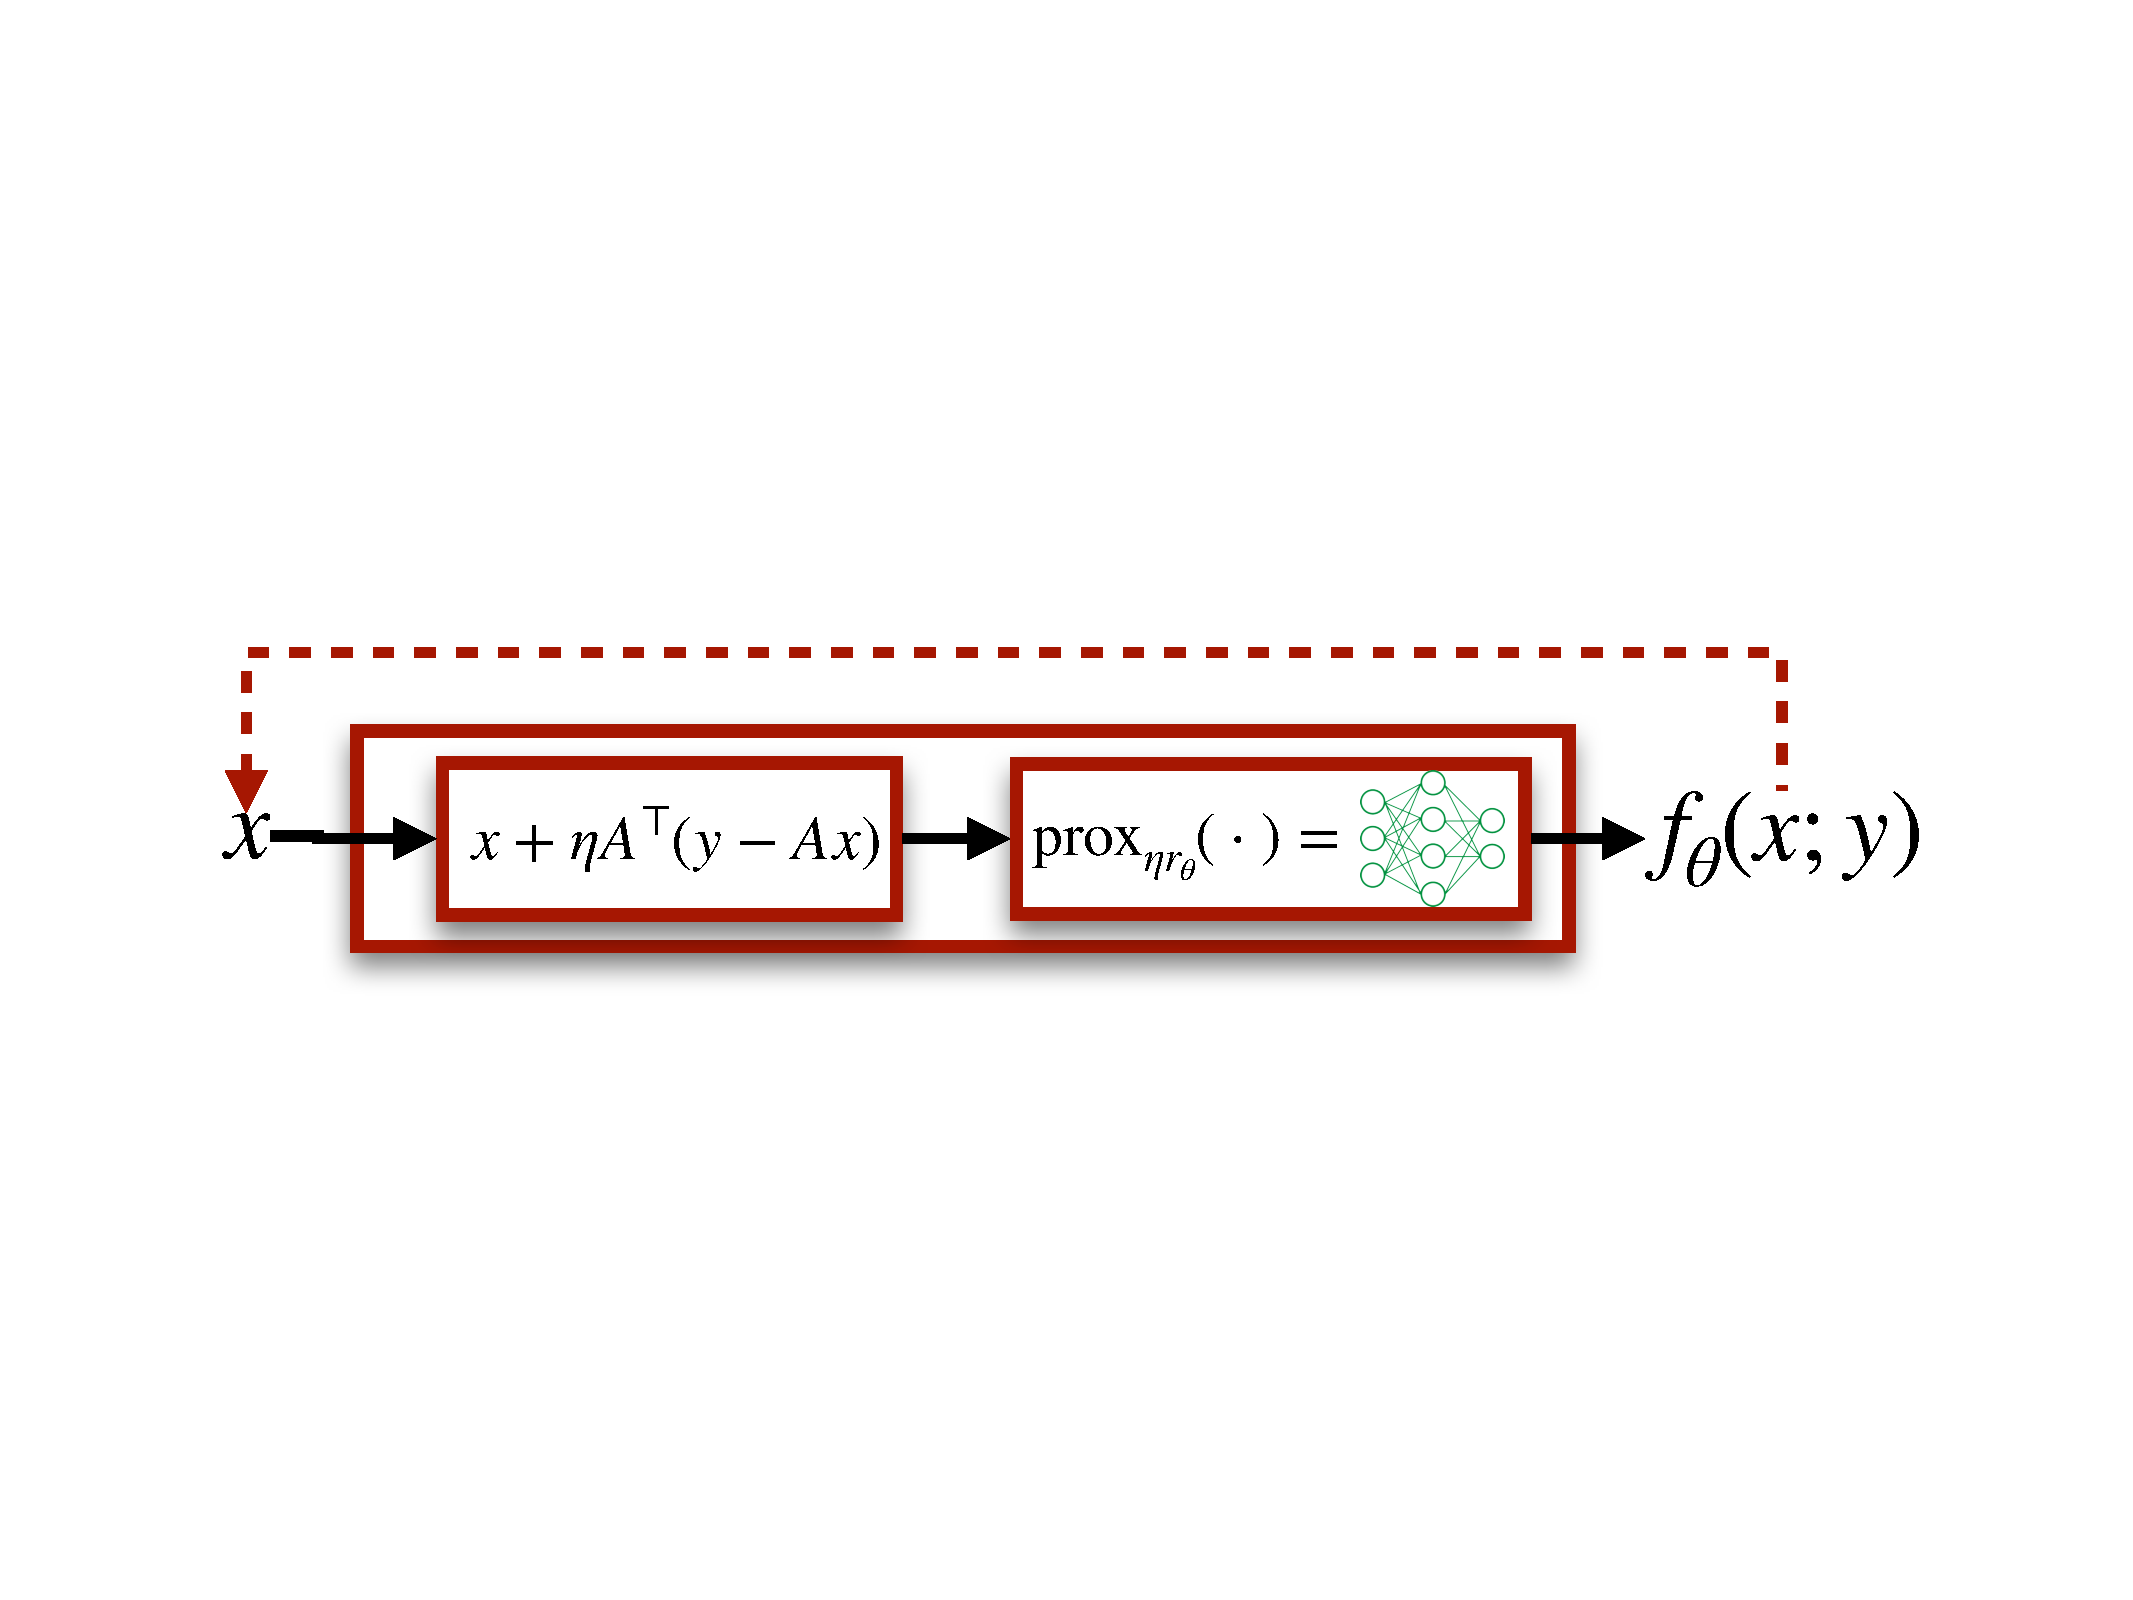
\includegraphics[width=0.6\textwidth]{../Common_Images/deq/DEProx.pdf}
    \caption{Architecture of the Deep Equilibrium Proximal Gradient Descent (DE-PROX) model. The model computes the equilibrium state of an iterative process involving a data-consistency gradient step followed by a learned regularisation block $R_\theta(\cdot)$. From \cite{gilton2021deep}.}
    \label{fig:deprox}
\end{figure}

\paragraph{DE-ADMM: equilibrium version of ADMM splitting}
Recall the ADMM updates for constrained splitting (see Algorithm \ref{alg:admm} from Chapter \ref{ch:unrolling}). If we again consider the variational problem in constrained form, i.e.
\begin{equation*}
    \min_{u,z} \; \frac{1}{2}\|f^\delta-Ku\|_2^2 + \alpha J(z) \quad \text{s.t.} \quad z=u,
\end{equation*}
the ADMM updates read as
\begin{align*}
z^{k+1}&=\operatorname{prox}_{\alpha J}(u^k-\zeta^k),\\
u^{k+1}&=(I+\alpha K^\top K)^{-1}\bigl(\alpha K^\top f^\delta + z^{k+1}+\zeta^k\bigr),\\
\zeta^{k+1}&=\zeta^k+z^{k+1}-u^{k+1}.
\end{align*}
DE-ADMM replaces $\operatorname{prox}_{\alpha J}$ by $R_\theta$ and interprets the resulting recursion as a fixed-point map on the joint state $q=(u,\zeta)$, i.e.,
\begin{equation*}
    q^{k+1}=f_\theta(q^k;f^\delta), \qquad q^\infty=f_\theta(q^\infty;f^\delta).
\end{equation*}
This gives an equilibrium architecture that preserves the splitting structure (primal and dual variables) of ADMM while learning the regularisation action end-to-end.

\paragraph{Convergence guarantees via contractive maps}
The DEM analysis in \cite{gilton2021deep} assumes a residual-Lipschitz condition of the form
\begin{equation*}
    \|(R_\theta-I)(u)-(R_\theta-I)(u')\| \leq \varepsilon \|u-u'\|,
\end{equation*}
and establishes contractivity of the induced iteration maps under explicit parameter conditions. With
\begin{equation*}
    L=\lambda_{\max}(K^\top K), \qquad \mu=\lambda_{\min}(K^\top K),
\end{equation*}
DE-GRAD is contractive for $\eta < 1/(L+1)$, with Lipschitz factor bounded by
\begin{equation*}
    \gamma = 1-\eta(1+\mu)+\eta\varepsilon,
\end{equation*}
and therefore convergent when $\gamma<1$ (e.g., $\varepsilon<1+\mu$). For DE-PROX, contractivity holds when
\begin{equation*}
    \frac{1}{\mu(1+1/\varepsilon)} < \eta < \frac{2}{L}-\frac{1}{L(1+1/\varepsilon)},
\end{equation*}
with feasibility condition $\varepsilon < 2\mu/(L-\mu)$. For DE-ADMM, a sufficient condition is
\begin{equation*}
    \alpha > \frac{\varepsilon}{(1+\varepsilon-2\varepsilon^2)\mu}.
\end{equation*}
These results formalise why DEM inference can be run to convergence, unlike fixed-depth unrolling. As discussed in \cite{gilton2021deep}, DE-PROX and DE-ADMM additionally assume $\mu>0$ (trivial nullspace), which is stricter than typical MRI/CS settings, but convergence is still observed empirically in undersampled regimes.

\paragraph{Empirical behaviour and computational trade-offs}
Across deblurring, compressed sensing, and accelerated MRI, DEM variants consistently improve PSNR/SSIM relative to matched deep-unrolled counterparts in \cite{gilton2021deep}. Representative gains include: CS ($4\times$) where DE-ADMM reaches $31.64$ dB (vs. $29.09$ dB for DU-ADMM); MRI ($8\times$) where DE-GRAD reaches $32.01$ dB (vs. $31.13$ dB for DU-GRAD); and MRI ($4\times$) where DE-ADMM reaches $33.72$ dB (vs. $32.56$ dB for DU-ADMM). Figure \ref{fig:mri_reconstruction} illustrates the resulting reconstruction quality for $8\times$ accelerated MRI. Crucially, iteration-vs-PSNR curves show that DU-Prox is sharply optimised near its training depth (e.g., $L=10$), while DE methods maintain or improve quality over a broader iteration range (see Figure \ref{fig:results_cs}). This enables a practical accuracy-time knob at test time: one may stop early for speed, or continue solving for improved fidelity, without the out-of-distribution iterate artefacts typical of finite unrolling.

\begin{figure}[htpb]
    \centering
    \begin{minipage}{0.24\textwidth}
        \centering
        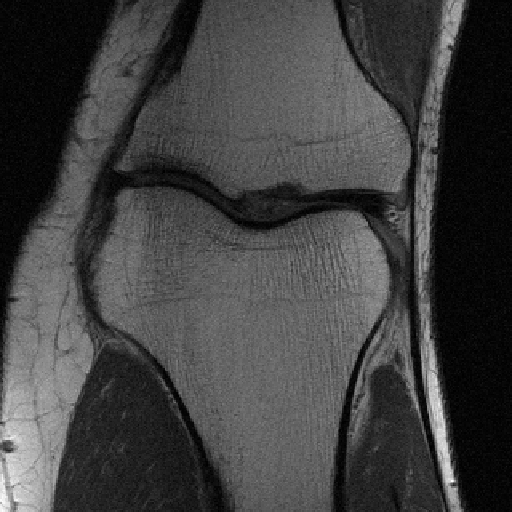
\includegraphics[width=\textwidth]{../Common_Images/deq/groundtruth_mri.png}
        \caption*{Ground truth}
    \end{minipage}
    \hfill
    \begin{minipage}{0.24\textwidth}
        \centering
        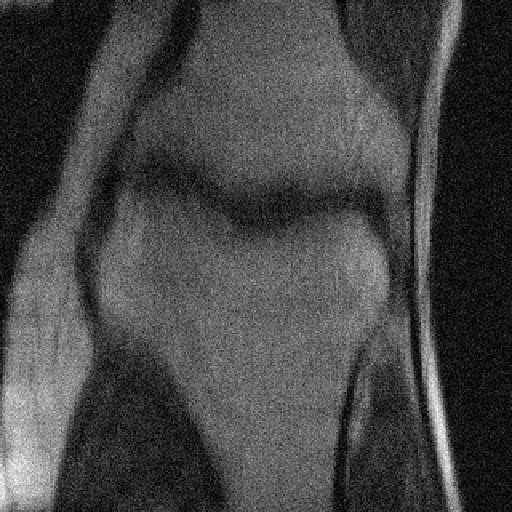
\includegraphics[width=\textwidth]{../Common_Images/deq/ifft_mri_8.png}
        \caption*{IFFT (24.53 dB)}
    \end{minipage}
    \hfill
    \begin{minipage}{0.24\textwidth}
        \centering
        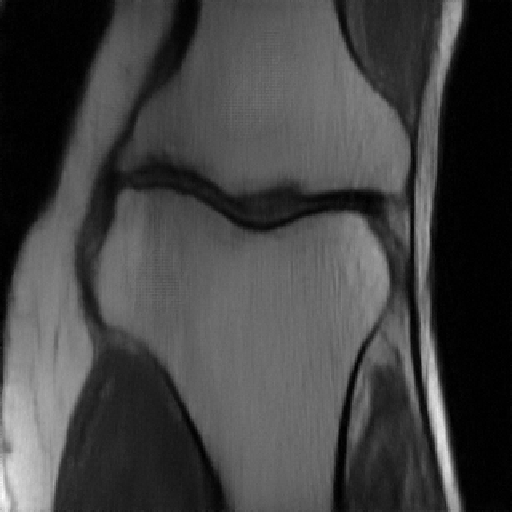
\includegraphics[width=\textwidth]{../Common_Images/deq/duprox_8_31.018515.png}
        \caption*{DU-PROX (31.02 dB)}
    \end{minipage}
    \hfill
    \begin{minipage}{0.24\textwidth}
        \centering
        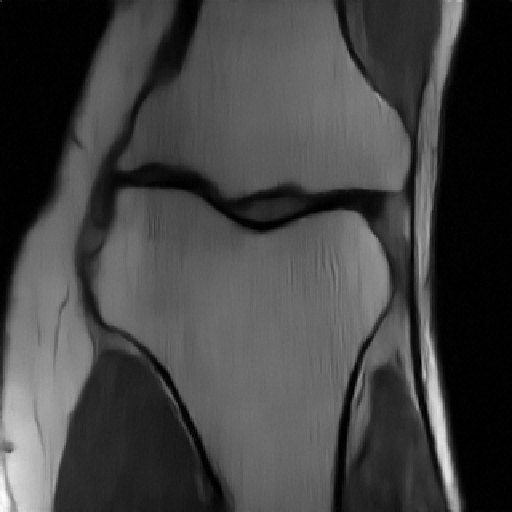
\includegraphics[width=\textwidth]{../Common_Images/deq/deprox_8_32.087868.png}
        \caption*{DE-PROX (32.09 dB)}
    \end{minipage}
    \caption{Visual comparison of $8\times$ accelerated MRI reconstruction. The deep equilibrium model (DE-PROX) produces sharper details and achieves higher PSNR compared to finite unrolling (DU-PROX) and the standard inverse Fourier transform. From \cite{gilton2021deep}.}
    \label{fig:mri_reconstruction}
\end{figure}

\begin{figure}[htpb]
    \centering
    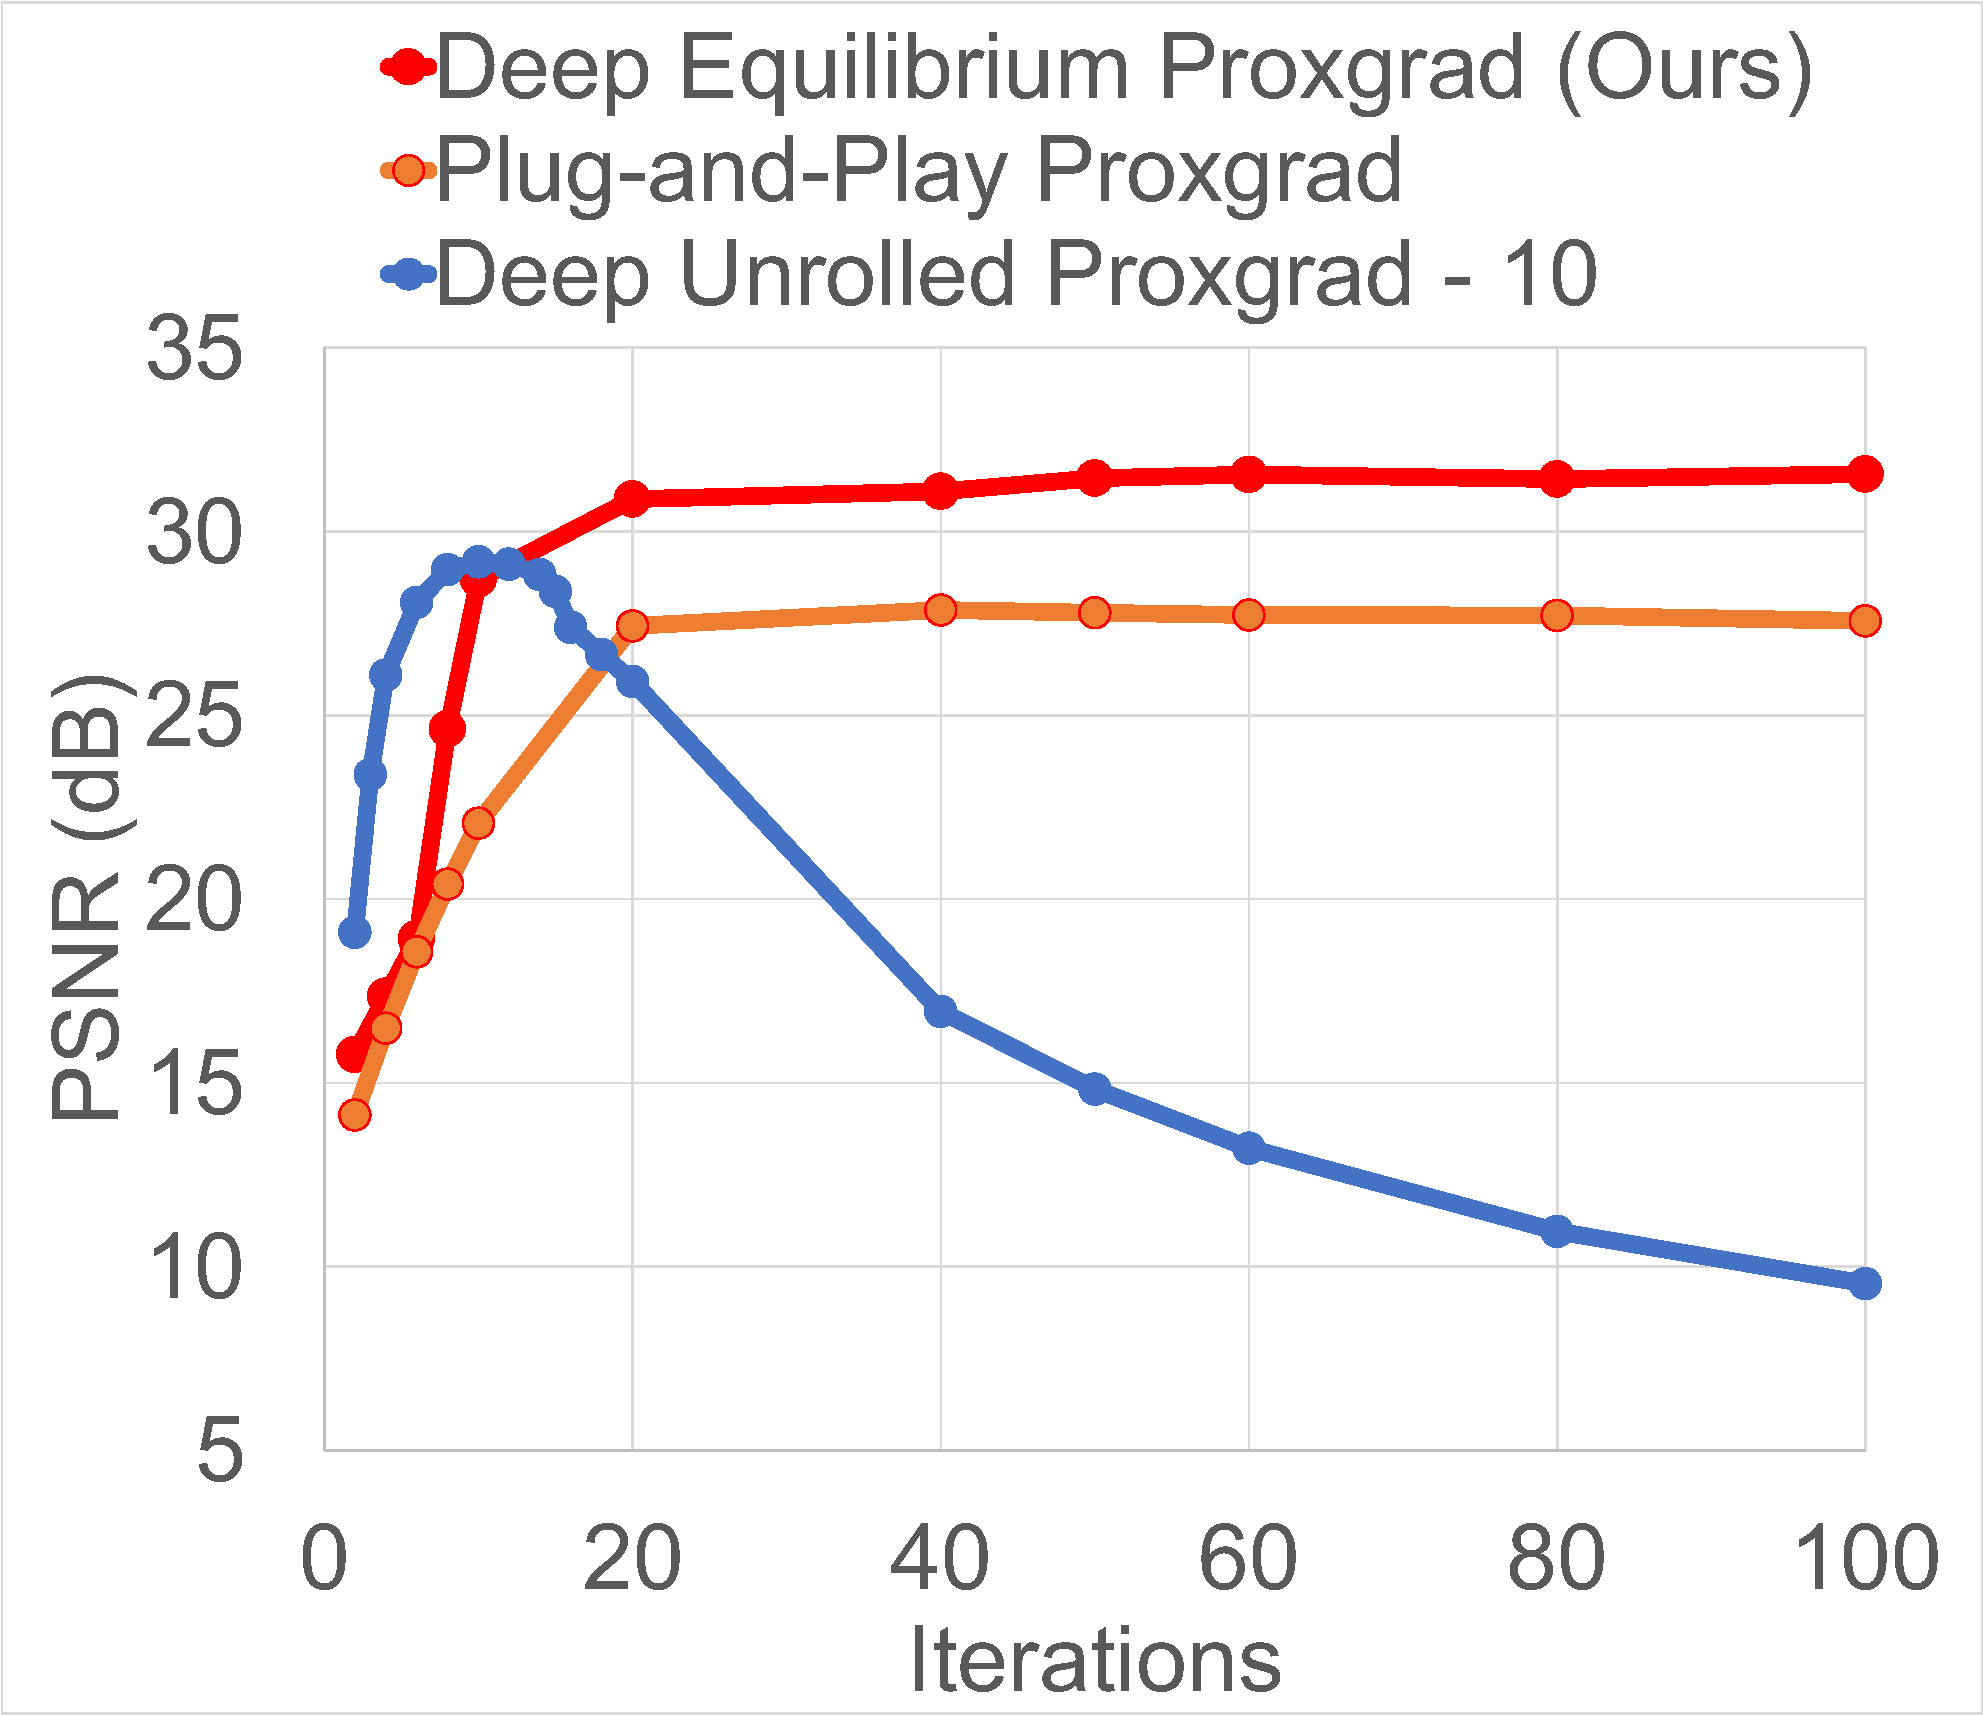
\includegraphics[width=0.6\textwidth]{../Common_Images/deq/ResultsCS.pdf}
    \caption{Iterations vs. reconstruction PSNR for DE-PROX and competing methods for compressed sensing. Deep unrolling is primarily effective at the number of iterations for which it is trained, whereas the deep equilibrium method achieves higher PSNR across a broad range of iterations. From \cite{gilton2021deep}.}
    \label{fig:results_cs}
\end{figure}

\section{Theoretical Link: DEQs versus Bilevel Learning}\label{sec:deq_vs_bl}
An alternative paradigm for data-driven inverse problems is bilevel learning as introduced in Section \ref{sec:bilevel}, which aims to learn a regulariser such that the minimiser of the resulting variational problem closely matches the ground-truth data. This requires solving an upper-level risk minimisation problem constrained by a lower-level variational problem (cf. \cite{riccio2022regularization}).

\subsection{Bilevel Optimisation formulation}
Given a training set of ground-truth images $(u_i^\dagger)$ and noisy measurements $(f_i^\delta)$, bilevel learning seeks parameters $\Psi$ that minimise an upper-level loss $\mathcal{L}$, such as the mean squared error, subject to a lower-level optimality condition. Problem \ref{prob:optimal_filter} in Chapter \ref{ch:data-driven} was already a specialised instance of this, where we learned spectral filter coefficients. In the general setting as introduced in Section \ref{sec:bilevel}, the formulation reads
\begin{equation*}
    \min_\Psi \frac{1}{N} \sum_{i=1}^N \mathcal{L}(u_i^\star(\Psi), u_i^\dagger) \quad \text{subject to} \quad u_i^\star(\Psi) \in \arg\min_u \left\{ \frac{1}{2}\|Ku - f_i^\delta\|_2^2 + \mathcal{R}_\Psi(u) \right\}.
\end{equation*}
When the parameterised regulariser $\mathcal{R}_\Psi$ is chosen such that the lower-level objective is strongly convex and differentiable, the unique minimiser $u^\star(\Psi)$ is fully characterised by the first-order optimality condition
\begin{equation*}
    K^\top(K u^\star - f^\delta) + \nabla \mathcal{R}_\Psi(u^\star) = 0.
\end{equation*}

\subsection{Bilevel Learning as a Restricted DEQ}
The authors of \cite{riccio2022regularization} discussed how bilevel learning schemes can be viewed as a subclass of Deep Equilibrium Models. The connection arises by observing that the solution to the lower-level variational problem, $u^\star(\Psi)$, is naturally a fixed point of some optimisation operator. For instance, if one solves the lower-level problem via gradient descent, the optimal solution satisfies the fixed-point equation
\begin{equation}
    u^\star = u^\star - \eta \left( K^\top(K u^\star - f^\delta) + \nabla \mathcal{R}_\Psi(u^\star) \right).
\end{equation}
Alternatively, one might use a proximal gradient step if $\mathcal{R}_\Psi$ is non-smooth. In either case, the bilevel problem is equivalent to learning the parameters $\Psi$ of an equilibrium model defined by
\begin{equation}
    f_\Psi(u; f^\delta) := u - \eta \nabla \Phi(u, f^\delta; \Psi),
\end{equation}
where $\Phi$ is the lower-level objective.

The key distinction is that in bilevel learning, the fixed-point map $f_\Psi$ is structurally constrained to be the update step of an optimisation algorithm minimising a potential function. In contrast, general DEQs learn a map $f_\theta$ that need not correspond to any energy minimisation process.

Riccio et al. \cite{riccio2022regularization} theoretically and empirically compare these frameworks. They show that while bilevel formulations offer strong interpretability (since the learned object is a regulariser within a clean variational energy), DEQs offer greater flexibility. By removing the constraint that the update field is a conservative vector field (a gradient), DEQs can learn more effective fixed-point dynamics. Empirically, \cite{riccio2022regularization} demonstrates that DEQ counterparts to bilevel models -— specifically DE-PROX versus bilevel learning of a convex regulariser—often achieve higher restoration quality and are more robust to hyperparameter tuning (as seen in Figure \ref{fig:deq_vs_bl_boxplot}), although bilevel models remain attractive for their rigorous variational interpretation. Figure \ref{fig:riccio_visual_comparison} shows a visual comparison highlighting that both approaches can still yield good restorations under optimal configurations. Thus, DEQs can be seen as a potentially larger class of models that includes bilevel learning as a specific, integrability-constrained subfamily.

\begin{figure}[htpb]
    \centering
    \begin{minipage}{0.48\textwidth}
        \centering
        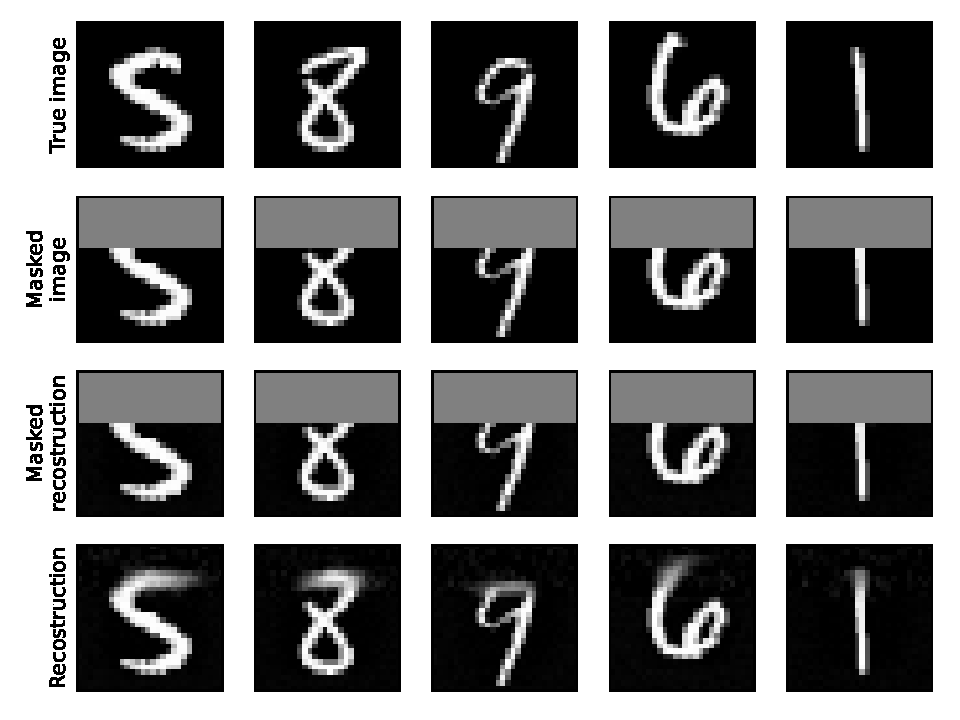
\includegraphics[width=0.9\textwidth]{../Common_Images/deq/riccio_inpainting_bl_test.pdf}
        \caption*{Bilevel Learning (BL)}
    \end{minipage}
    \hfill
    \begin{minipage}{0.48\textwidth}
        \centering
        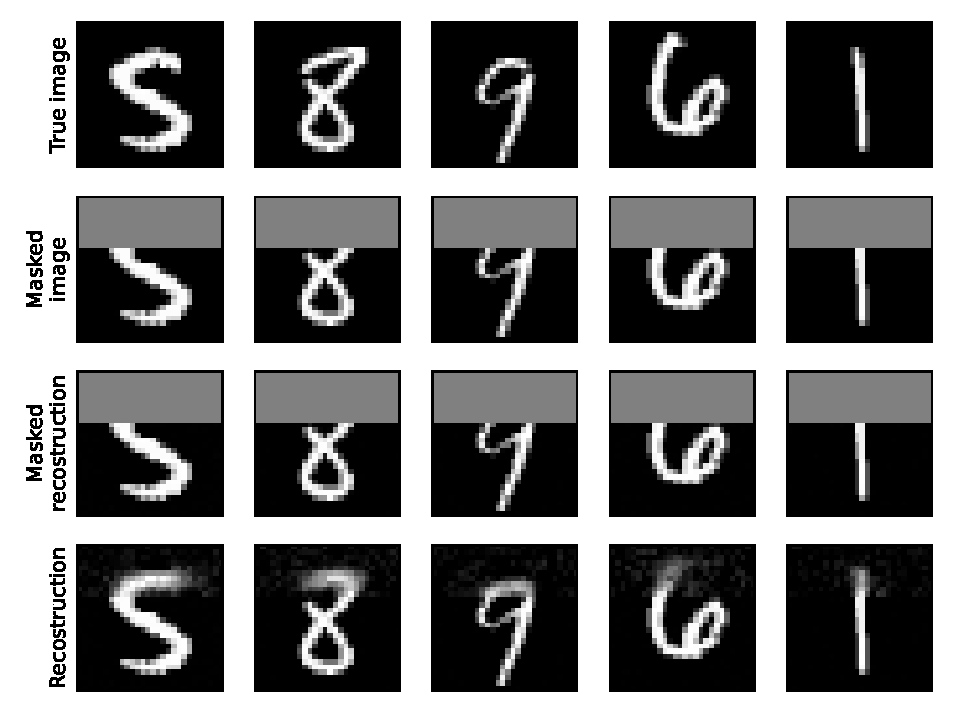
\includegraphics[width=0.9\textwidth]{../Common_Images/deq/riccio_inpainting_deq_test.pdf}
        \caption*{Deep Equilibrium (DEQ)}
    \end{minipage}
    \caption{Qualitative results for the inpainting task on the MNIST dataset. The original image (top row) is partially masked (second row) and the task is to recover the missing pixels. The output of the models (bottom row) indicates that both the integrability-constrained bilevel framework and the unconstrained deep equilibrium method successfully reconstruct the image, with DEQs offering more flexible update operators. From \cite{riccio2022regularization}.}
    \label{fig:riccio_visual_comparison}
\end{figure}

\begin{figure}[htpb]
    \centering
    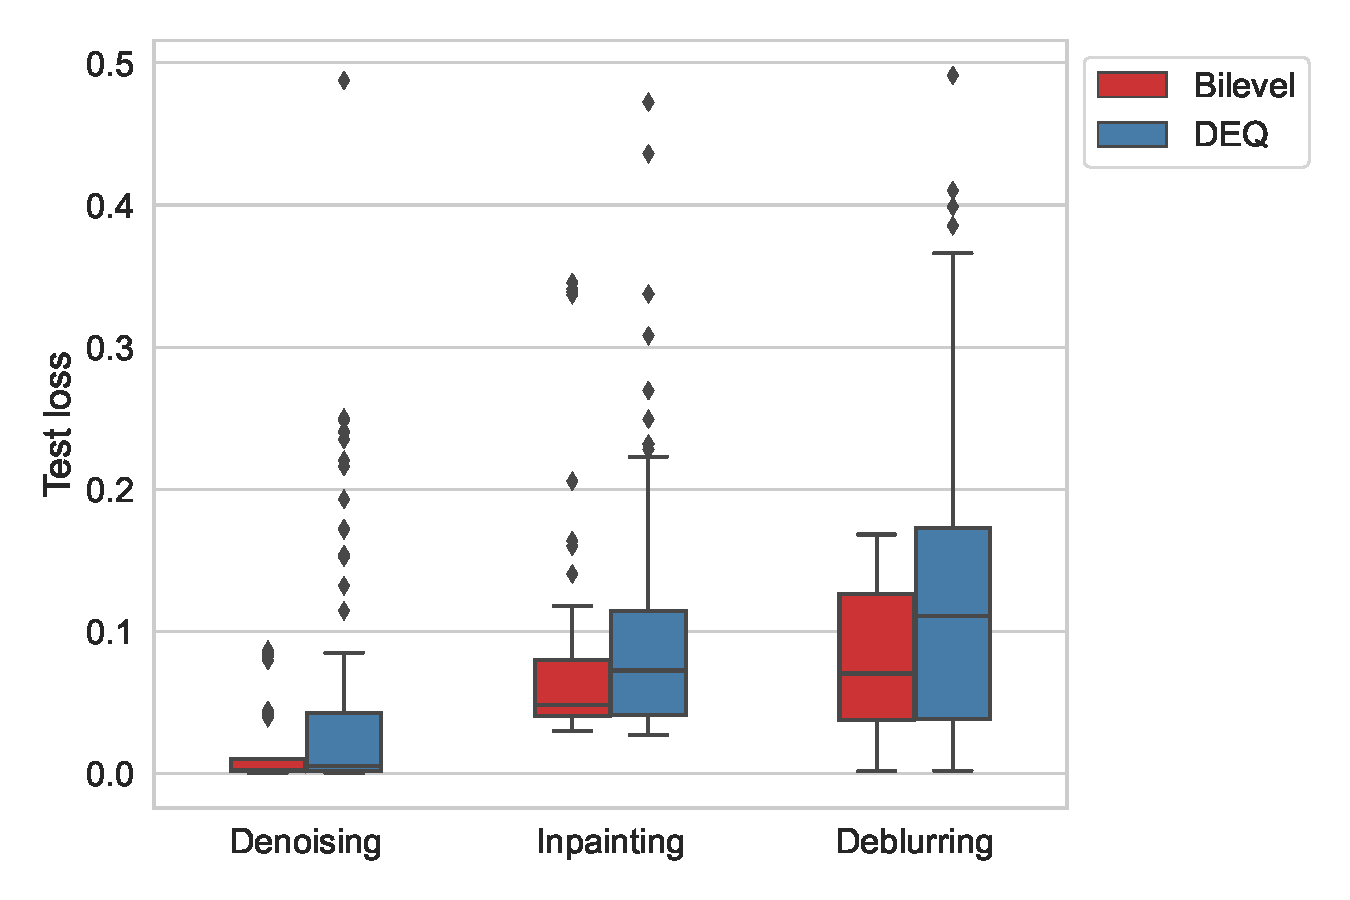
\includegraphics[width=0.7\textwidth]{../Common_Images/deq/boxplot_comparison_tasks.pdf}
    \caption{Comparison between bilevel optimisation (BL) and deep equilibrium models (DEQ) across denoising, inpainting, and deblurring tasks. The boxplots illustrate the loss of the trained models evaluated on the test dataset across various hyperparameter configurations, demonstrating the general performance advantage of DEQs, but robustness advantage of Bilevel learning. From \cite{riccio2022regularization}.}
    \label{fig:deq_vs_bl_boxplot}
\end{figure}
